\documentclass[]{spie}  %>>> use for US letter paper
%\documentclass[a4paper]{spie}  %>>> use this instead for A4 paper
%\documentclass[nocompress]{spie}  %>>> to avoid compression of citations

\renewcommand{\baselinestretch}{1.0} % Change to 1.65 for double spacing

\usepackage{amsmath,amsfonts,amssymb} \usepackage{graphicx}
\usepackage[colorlinks=true, allcolors=blue]{hyperref}


\usepackage{color} \usepackage[latin9]{inputenc} \usepackage{mathrsfs,amsmath}
\usepackage{graphicx}% \usepackage{float} \usepackage{amsfonts}%
\usepackage[titletoc]{appendix} \usepackage{amssymb} \usepackage{braket}
\usepackage{bm}

\newcommand{\mb}[1]{\bm{#1}} \usepackage[T1]{fontenc}

\def\Nabla{\bm{\nabla}} \def\bm{\mathbf} \def\curl{\Nabla\times}
\def\div{\Nabla\cdot} \def\lap{\Delta} \def\vlap{\Delta} \def\x{\hat{e}_{x}}
\def\y{\hat{e}_{y}} \def\z{\hat{e}_{z}} \def\p{\partial} \def\h{\hat}
\def\h{\hat} \def\tw{\tilde{\omega}} \def\gm{\gamma} \def\om{\omega}
\def\OM{\Omega} \def\GM{\Gamma} \def\dw{\delta\omega} \def\dth{\Delta\theta}
\def\dk{\delta k} \def\Hdth{\frac{\dth}{2}} %half Delta Theta

\def\width{10cm} \title{Temporal Hole Burning in QCLs - derivation}


\author[a]{Petar Tzenov} \date{June 6, 2016}%

\authorinfo{Further author information:\\a: E-mail: petar.tzenov@tum.de}

% Option to view page numbers
\pagestyle{empty} % change to \pagestyle{plain} for page numbers
\setcounter{page}{301} % Set start page numbering at e.g. 301

\begin{document} \maketitle
	
	


\begin{abstract} The abstract is the last section of your article to be written
 	because it is a condensed version of the entire article. It includes the key
 	points of the introduction, methods and results, and conclusions. An abstract
 	is generally 100?250 words long. It is written in the past tense. An abstract
 	should not include references; use the background and conclusions to help frame
 	the context of your work [9].  Readers will use the abstract to decide if your
 	article is relevant to them. Use keywords and index terms in your abstract to
 	capture reader interest and improve the likelihood of your article appearing in
 	relevant searches [3]. Readers who find your article through an abstracting
 	service may never see the rest of your article. Be sure the abstract conveys
 	why your research problem is important and how your work moves the field
 	forward.  Reviewers also look at the abstract first. Strive to make a good
 	impression with your abstract to engage their attention.  \end{abstract}

% Include a list of keywords after the abstract 

\section{Introduction} \begin{itemize} 
\item {Short introduction to spatial and spectral hole burning.
	 Sell this as the last out of a group of effects} \item
 	{Short description of the problem formulation -> where was it first reported
 		and what are the specific characteristics of THB} 
\end{itemize} 
The Introduction serves to help the reader understand our three key questions: Why
is this a new and important problem?  What has been done before? How does your
research bring significant new understanding to the field? The reader should
find enough information to understand why your research was necessary, without
having to refer to other source material or published works [7]. The
introduction should be concise, no more than one or two pages. It is written in
the present tense.  Your introductory paragraph should start with what is
generally known about your subject. Then move step by step through more
detailed information, ending with a description of the specific problem or
hypothesis your article will discuss. Try to use an attention-grabbing
statement to hook the reader [10] while being careful not to sensationalize
your results.  In the next few paragraphs, refer to the published research to
show what is already known about your subject and why your work is needed. Do
not try to include everything from your literature review. Your goal is to
orient the reader to the most relevant studies. Explain how each earlier study
relates to your own approach to the problem. Does it have limitations? Does it
make different assumptions [11]? Show your readers how your study builds upon
or is different from this existing work. If you have published an earlier
version of your work, for example as a conference or journal article, you must
explain how the current study builds upon your own prior work [3].  After you
have explained the historical context of your work, introduce your hypothesis
and provide a general description of the results you have obtained. You will
flesh these out more fully later in the article, but providing an overview here
motivates your audience to read on. At the end of your introduction, tell the
reader how the article is organized. This will allow readers to move to
sections of particular interest, if they wish.  \section{Experimental evidence}

In addition to emitting a stable frequency comb, consisting of more than 70
equidistantly-spaced longitudinal modes, the device in
\cite{burghoff2014terahertz} also exhibited other very intriguing properties
which deserve a more detailed study. For example, a hole was observed in the
signal's spectrum, which separated the lasing frequencies into components
distributed around 3.4 THz and 3.8 THz, to which we will refer  as the low and
high frequency lobes, respectively. Such a spectral hole burning was attributed
and later theoretically confirmed by simulation [cite our optics paper] to be
due to the strong tunneling coupling between injector and upper laser level of
the active region. Furthermore, a subsequent detailed experimental analysis
\cite{burghoff2015evaluating} showed that the prevalent frequency lobe strongly
depends on the applied injection current, with the low and high frequency
transitions dominating respectively at low and high current densities
\cite{burghoff2015evaluating}. Additionally, a Monte-Carlo based algorithm in
combination with a novel comb coherence detection technique, the so called
shifted wave interference Fourier transform spectroscopy or SWIFTS
\cite{burghoff2014broadband}, was used in order to reconstruct the
instantaneous intensity and frequency of the signal
\cite{burghoff2015evaluating}. The results displayed an intriguing pulse
switching behaviour, which was termed "temporal hole burning" (THB) by the
authors, and is at the main focus of this article.  The observed THB effect can
be characterized by a transient switching between signals corresponding to the
high and low lobes in a manner as to maintain an almost constant total
intensity. This process is illustrated in Fig. \ref{fig:img01}b which displays
experimental data of the averaged out instantaneous intensity of the low and
high frequency lobes of the power spectrum in Fig. \ref{fig:img01}a. For this
measurement the laser was supplied with 0.9 A current and was shown to operate
in a stable comb regime. From the plots in Fig. \ref{fig:img01}, we immediately
see that whereas both signals' intensities are comparable in strength, the high
frequency lobe has significantly longer time duration and hence carries more
power. In agreement with Parseval's theorem, this is also confirmed by the
optical power spectrum in Fig. \ref{fig:img01}a, where we see that
significantly more energy is stored in the modes distributed around 3.8 THz as
compared to those at 3.4 THz.  \begin{figure}[h!] \begin{center}
 		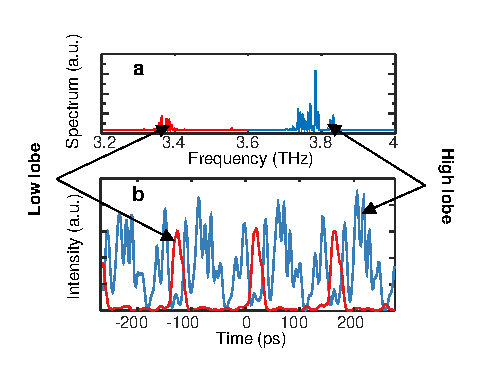
\includegraphics[width=10cm]{THB_experiment.eps} \caption{ Insert Caption HERE}
 		\label{fig:img01} \end{center}	\end{figure}


\section{Density matrix equations in the dressed states basis}
\label{sec:biasdependence}

The introduction of the coupling energy $\hbar \Omega_{1'3}$ into the
Hamiltonian of the system contributes to a splitting of the optical spectra
into a high and a low frequency lobes. This is due to the fact that the
original system's Hamiltonian is non-diagonal in the tight binding basis. The
new eigenstates, which in the absence of electromagnetic radiation, i.e.
$f(x,t) \approx 0$, diagonalize the Hamiltonian in Eq.
(\ref{eq:hamiltonian-operatorform}), are the so called delocalized, or dressed,
states and are obtained from the tunneling levels $\Ket{1'}$ and $\Ket{3}$ via
the unitary transformation \begin{align} \label{eq:dressedstates} \Ket{+} &=
\cos\theta \Ket{1'} - \sin\theta \Ket{3}, \nonumber \\ \Ket{-} &= \sin\theta
\Ket{1'} + \cos\theta \Ket{3}.  \end{align} The corresponding energies are
given by $E_\pm =\hbar(\omega_0 +\epsilon/2) \pm \hbar
\left(\epsilon^2+4\Omega_{1'3}^2\right )^{1/2}$, and the expansion coefficients
are computed from   $ \tan \theta =
-2\Omega_{1'3}/[\epsilon+(\epsilon^2+4\Omega_{1'3}^2)^{1/2}].  $ Within the
full extended basis picture, where the wave functions are calculated for
several neighbouring periods, these tight-binding states are simply split
electron states spanning the intermodule barrier, see Fig.
\ref{fig:basis_schemata}b. Both dressed states  couple radiatively to the lower
laser level $\ket{2}$, since they both have a component in the $\ket{3}$
direction in the tight binding expansion. We can calculate the ratio of the
dipole matrix elements for the $\Ket{+}\leftrightarrow\Ket{2}$ and
$\Ket{-}\leftrightarrow\Ket{2}$ transitions, which will determine the relative
strength between the high and low frequency lobes of the gain. If we assume
that the $d_{1'2} \approx 0$, which is reasonable in the tight binding basis
due to the negligible overlap between wave function in different modules, we
obtain  $|\Bra{+}\hat{z}\Ket{2}|/|\Bra{-}\hat{z}\Ket{2} | \approx |\tan\theta|
=  2|\Omega_{1'3}|/|\epsilon+\sqrt{\epsilon^2+4\Omega_{1'3}^2}|$. We now can
see that at positive detunings $\epsilon >0$, $|\tan\theta|<1$ and thus the low
frequency transition will have higher probability. On the other hand, for
$\epsilon < 0 $ we get that $|\tan\theta| >1$ which will lead to lasing
predominantly in the high frequency regime.

\begin{figure}[h!] \begin{center}
 		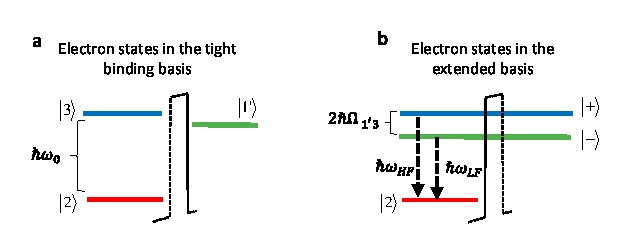
\includegraphics[width=10cm]{BASISPICTURE.eps} \caption{ Schematic illustration
 			of the tight binding \textbf{a} and extended basis \textbf{b}, states.  }
 		\label{fig:basis_schemata} \end{center}	\end{figure} \section{Extended basis
 	EOM} Within the delocalized basis picture the observed pulse switching
behaviour has a very intuitive and simple explanation. If we apply the unitary
transform given by Eq. (\ref{eq:dressedstates}) onto the tight binding
Hamiltonian and also employ the rotating wave approximation, the Hamiltonian
and the statistical operator can be cast in the following matrix form
\begin{equation} H^{\text{RWA}} = \begin{bmatrix} \hbar (\omega_+-\omega_c) & 0
& q_0d_{+2}f/2 \\ 0 & \hbar (\omega_--\omega_c) & q_0d_{-2}f/2 \\
q_0d_{+2}f^*/2 & q_0d_{-2}f^*/2 & 0 \\ \end{bmatrix},\quad \rho^{\text{RWA}} =
\begin{pmatrix} \rho_{++} & \rho_{+-} & \eta_{+2} \\ \rho_{-+} & \rho_{--} &
\eta_{-2} \\ \eta_{2+} & \eta_{2-} & \rho_{22} \\ \end{pmatrix}.
\end{equation} The symbols $d_{+2} = \Bra{+}\hat{z}\Ket{2} $ and $d_{-2} =
\Bra{-}\hat{z}\Ket{2} $, denote the corresponding dipole moments, and $
\eta_{\pm 2}$ the slowly varying coherences. 

In this basis, the von Neumann equation reads (neglecting collision terms)
\begin{subequations} \begin{align} \frac{d \rho_{++}}{dt} &=
 	i\frac{q_0d_{+2}}{2\hbar}(f^*\eta_{+2}-f\eta_{+2}^*), \\ \frac{d \rho_{--}}{dt}
 	&= i\frac{q_0d_{-2}}{2\hbar}(f^*\eta_{-2}-f\eta_{-2}^*), \\ \frac{d
 		\rho_{22}}{dt} &=
 	-i\frac{q_0d_{+2}}{2\hbar}(f^*\eta_{+2}-f\eta_{+2}^*)-i\frac{q_0d_{-2}}{2\hbar}(f^*\eta_{-2}-f\eta_{-2}^*),
 	\\ \frac{d \rho_{+-}}{dt} &=
 	-i(\omega_+-\omega_-)\rho_{+-}-i\frac{q_0d_{+2}}{2\hbar}f\eta_{2-}+i\frac{q_0d_{-2}}{2\hbar}f^*\eta_{+3},\\
 	\frac{d \eta_{+2}}{dt} &=
 	-i(\omega_+-\omega_0)\eta_{+2}+i\frac{q_0d_{+2}}{2\hbar}f(\rho_{++}-\rho_{22})+i\frac{q_0d_{-2}}{2\hbar}f\rho_{+-},
 	\label{eq:eta+2}\\ \frac{d \eta_{-2}}{dt} &=
 	-i(\omega_--\omega_0)\eta_{-2}+i\frac{q_0d_{-2}}{2\hbar}f(\rho_{--}-\rho_{22})+i\frac{q_0d_{+2}}{2\hbar}f\rho_{-+}.
 	\label{eq:eta-2} \end{align} \end{subequations} Now, if we assume that $f =
f^*$,  $\epsilon \approx 0$ and also that $d_{+2}\approx d_{-2} = d$, it turns
out that we can reduce the $3-$level delocalized state system into a
quasi-2-level system, by setting  $\eta = \eta_{+2}+(\eta_{-2})^*$ and deriving
the time evolution of this quantity. Adding Eq. (\ref{eq:eta+2}) with the
complex conjugate of Eq. (\ref{eq:eta-2}), we obtain \begin{equation}
\label{eq:coherence_quasi2lvl} \frac{d \eta}{dt} = -2i\Omega_{1'3} \eta +
i\frac{q_0d}{2\hbar}fw, \end{equation} where $w = \rho_{++}-\rho_{--}$ denotes
the inversion between the delocalized states, which	 evolves according to
\begin{align} \label{eq:inversion_quasi2lvl} \frac{d w }{dt}	&=
i\frac{q_0d}{2\hbar}f(\eta-\eta^*).  \end{align} We thus see that under the
above idealized assumptions, we have reduced the three level system into an
effective two level such. In fact, this is a "quasi" two level system due to
the presence of a factor of 2 in the denominator of Eq.
(\ref{eq:inversion_quasi2lvl}), which distinguishes it from the standard Bloch
equations \cite{boyd2003nonlinear}.

To see why Eqs. (\ref{eq:coherence_quasi2lvl}) and
(\ref{eq:inversion_quasi2lvl}) could lead to a pulse switching behaviour we
need to include the optical field propagation equations into the model. For
classical fields, absence of free electric charges and weak inhomogeneities,
the electric field envelope (within the slowly varying amplitude approximation)
obeys the propagation equation \begin{align} \frac{n_0}{c} \p_t f - \p_x f =
-i\frac{N \Gamma q_0d k_c}{\epsilon_0 n^2}(\eta_{+2}+\eta_{-2}), \end{align}
where $\epsilon_0$ is the permittivity of free space and $N$ is the average
carrier density per unit volume. Now decomposing the polarization envelopes,
$\eta_{+2}$ and $\eta_{-2}$ into their real and imaginary parts, i.e.
$\eta_{+2} = u_{+}+iv_{+}$ and $\eta_{-2} = u_{-}+iv_{-}$, and plugging into
the propagation equation we obtain that \begin{align}
\label{eq:field_propagation} \frac{n}{c} \p_t f - \p_x f = -i\frac{N \Gamma
 	q_0d k_c}{\epsilon_0 n^2}(u_{+}+u{-}) + \frac{N \Gamma q_0d k_c}{\epsilon_0
 	n^2}(v_{+}+v_{-}).  \end{align} The right hand side of Eq.
(\ref{eq:field_propagation}) has straightforward interpretation. While the real
part of the polarization is proportional to the change in the real part of the
refractive index, the imaginary parts capture the electric field loss/gain due
to the resonant transition. On the other hand, from the quasi two level system
Eq. (\ref{eq:inversion_quasi2lvl}), we see that the \emph{difference} of the
imaginary parts of the coherences, i.e. $v_{+}-v_{-} = \Im\{\eta\}$, has the
same time evolution. This means that the high frequency transition's gain
($\ket{+}\leftrightarrow\ket{2}$) and low frequency transition's
($\ket{-}\leftrightarrow\ket{2}$) loss form a co-propagating quasi particle and
vice versa. This intuitively explains how the coherent time evolution of the
quasi-two level system would lead to a pulse switching behaviour, which has
already been observed by experiment\cite{burghoff2015evaluating} and also
captured by our simulations.

Lastly, we will elaborate a little further in order to reveal the time
evolution of this quasi two level system by casting it into Bloch form. The
standard substitutions, $u=(\eta + \eta^*)/2$, $v = -i(\eta - \eta^*)/2$ and as
before $w = \rho_{++}-\rho_{--}$, in Eq. (\ref{eq:inversion_quasi2lvl}) and
(\ref{eq:coherence_quasi2lvl}), yield what we will call the "quasi-Bloch
equations" \begin{subequations} \label{eq:quasi-Blocheqn} \begin{align} \dot{u}
 	&= 2\Omega_{1'3} v , \\ \dot{v} &= -2\Omega_{1'3} u +\beta w , \\ \dot{w} &=
 	-2\beta v, \end{align} \end{subequations} where $\beta(t) = f(t)q_0d/2\hbar$ is
the Rabi frequency (for convenience we have dropped any $x-$dependence in the
ODEs). Notice that the above are \emph{not} the familiar Bloch equations due to
the presence of a factor of $2$ in the equation for $\dot{v}$ and therefore the
solutions (in the fully coherent case) do \emph{not} lie on the Bloch sphere of
radius 1. When we neglect dephasing, we can see that $d(u^2+v^2+w^2)/dt =
-2\beta vw \neq 0$ is actually not a conserved quantity.


Solving Eq. (\ref{eq:coherence_quasi2lvl}) and (\ref{eq:inversion_quasi2lvl}),
or equivalently Eq. (\ref{eq:quasi-Blocheqn}) numerically, reveals that the
system dynamics is governed by two time scales, one fast oscillating term with
a period close to $1/2\Omega_{1'3}$, which is driven by the beating between the
high and low frequency lobes, and another, slower time-scale the period of
which is seen to increase with the maximum magnitude of the Rabi frequency
$\beta(t) = q_0df(t)/2\hbar$. If we simply assume that $\beta(t) = \beta_0
\cos\omega_f t$, where $\omega_f$ is XXX, we find fact the system exhibits
strong resonance at $\omega_f = 2\Omega_{1'3}$. To illustrate that, we refer
the reader to Fig. \ref{fig:quasi-bloch-off-resonance} and Fig.
\ref{fig:quasi-bloch-resonance}.  \begin{figure}[h!] \begin{center}
 		\includegraphics[width=10cm]{quasi-bloch-off-resonance.eps} \caption{ Put
 			Caption Here } \label{fig:quasi-bloch-off-resonance} \end{center}
\end{figure} From Fig.  displays simulation results $\omega_f =
1.9\times\Omega_{1'3}$  $\omega_f = 2\Omega_{1'3}$.

\begin{figure}[h!] \begin{center}
 		\includegraphics[width=10cm]{quasi-bloch-resonance.eps} \caption{ Put Caption
 			Here } \label{fig:quasi-bloch-resonance} \end{center}	\end{figure}



\begin{figure}[h!] \begin{center} \includegraphics[width=10cm]{spheres.eps}
 		\caption{ Put Caption Here } \label{fig:spheres} \end{center}	\end{figure}


A few comments on the assumptions made in the above derivations are in order.
First of all, it will be interesting to consider when will the reality
condition for the envelope $f(x,t) $  hold. To investigate that, let us take an
input pulse $f_{in}(t_0) = f(x=0,t_0)$, with Fourier transform
$F_{in}(\omega)$, entering the medium at the left facet, such that at
$F_{in}(\omega)^* = F_{in}(-\omega)$, i.e. $f_{in}$ is real. After propagating
a distance $L$ inside the cavity the pulse transforms according to
\cite{weiner2011ultrafast} \begin{align} \label{eq:fout-expansion} f(x=L,t) &=
\int_{-\infty}^{\infty} F(x=L,\omega)e^{-i\omega t}d\omega =
\int_{-\infty}^{\infty} F_{in}(\omega)e^{-i\omega
 	t}e^{g(\omega)L+i\Psi(\omega)}d\omega, \end{align} where $g(\omega)$ denotes
the spectral gain per unit length and $\Psi(\omega)=k(\omega)L$, the acquired
phase. In order for $f(x=L,t)$ to remain real, it is sufficient that
$F(x=L,\omega)^*= F(x=L,-\omega)$. To find when this holds, we first expand the
wave number $k(\omega)$ around $\omega=0$ up to fourth order to get
\begin{align} \label{eq:k-expansion} k(\omega) = \beta_1\omega +
\frac{\beta_2}{2}\omega^2 + \frac{\beta_3}{6}\omega^3 + O(\omega^4),
\end{align} which is justified since, by virtue of the rotating wave
approximation, we had centred the spectrum around zero and also subtracted out
$\beta_0 = k_c$ as the wave number at the central frequency $\omega_c$. Now
from Eqs. (\ref{eq:fout-expansion}) and (\ref{eq:k-expansion}), we can write
(neglecting terms $\propto O(\omega^4)$) \begin{subequations} \begin{align}
 	F(x=L,\omega)^* &\approx F_{in}(\omega)^* \exp\{g(\omega)L-i(\beta_1\omega +
 	\frac{\beta_2}{2}\omega^2 + \frac{\beta_3}{6}\omega^3 )L\}, \\ F(x=L,-\omega)
 	&\approx F_{in}(-\omega) \exp\{g(-\omega)L+i(-\beta_1\omega +
 	\frac{\beta_2}{2}\omega^2 - \frac{\beta_3}{6}\omega^3 )L\}, \end{align}
\end{subequations} which will be equal if \begin{subequations} \begin{align}
g(-\omega) &= g(\omega), \label{eq:symmetric-gain}\\ \beta_2 = \beta_4 &= ... =
\beta_{2n}=0. \label{eq:vanish-even-order-dispersion} \end{align}
\end{subequations} The symmetric gain condition, Eq. (\ref{eq:symmetric-gain}),
will be satisfied when the device is biased at injector $\leftrightarrow$ upper
laser level resonance, as elaborated in Sec. \ref{sec:biasdependence}. On the
other hand Eq. (\ref{eq:vanish-even-order-dispersion}) requires vanishing even
order dispersion. We note that the comb in Ref. \cite{burghoff2014terahertz}
probably approximately satisfies this condition, due to the incorporation of a
dispersion compensation mechanism designed specifically to cancel the GVD
coefficient $\beta_2$.

\begin{figure}[h!] \begin{center}
		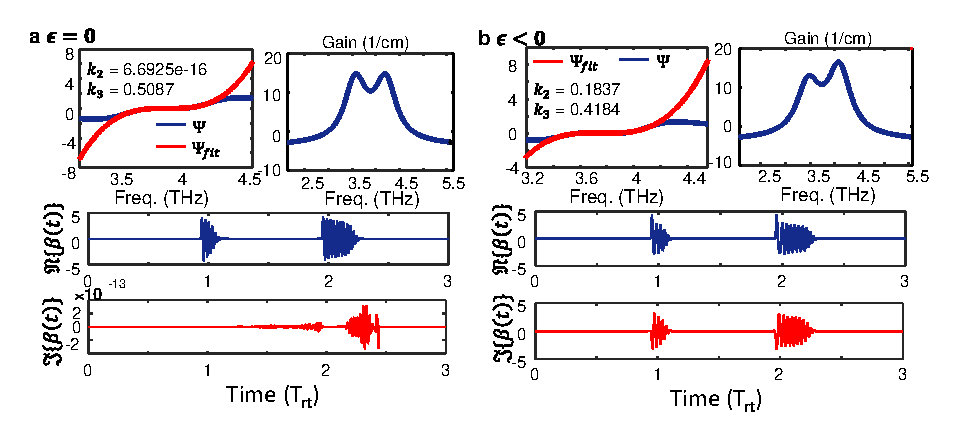
\includegraphics[width=10cm]{dispersion-on-off-resonance.eps} \caption{ Put
			Caption Here } \label{fig:dispersion-on-off-resonance} \end{center}
\end{figure}


Lastly, the second assumption we made was that the dipole moments have equal
algebraic value, i.e. $d_{+2} = d_{-2} = d$. What if they have opposite signs,
i.e. $d_{+2} = -d_{-2} = d$? It is very easy to show that one can derive an
equivalent quasi-two level system, but this time with the coherence set as
$\eta = \eta_{+2}-\eta_{-2}^*$, instead of the substitution made above. In this
case, the interpretation of the pulse switching behaviour remains the same, as
the reader can readily verify by him/her-self.  \acknowledgments % equivalent
to \section*{ACKNOWLEDGMENTS}       

% References
\bibliographystyle{spiebib} \bibliography{../../literature/bib_resources}


\end{document} 

